\chapter{Listas encadeadas}


As listas são estruturas de dados que permite que as operações inserção e remoção possam ser realizadas em tempo constante em qualquer posição da estrutura. 

As listas encadeadas podem ser:

\begin{itemize}
\item listas encadeadas simples.
\item listas duplamente encadeadas.
\end{itemize}


Nas listas encadeadas, temos apenas um link interno para o próximo elemento, enquanto nas listas duplamente encadeadas, temos um link para o próximo próximo e o anterior. Diferente das listas sequenciais, as listas encadeadas executam melhor as operações de inserção, remoção e movimentação dos elementos dentro da estrutura.

A principal desvantagem das listas encadeadas e duplamente encadeadas comparada com as listas sequencias e que elas não permitem o acesso direto para um elemento usando uma posição.
 



\section{Recursão em listas encadeadas}

O tipo \texttt{Node<T>} é um tipo recursivo contendo um ponteiro para o próximo nó da nossa lista encadeada e um valor val do tipo T.


\begin{minted}{C++}
template <typename T>
class ListNode {
    public:
    T val;
    ListNode *next;
    ListNode() : val( T()  ), next(nullptr) {}
    ListNode(T x) : val(x), next(nullptr) {}
    ListNode(T x, ListNode *next) : val(x), next(next) {} 
};
\end{minted}



\subsection{Tamanho de uma lista}

Dado o nó cabeça de lista encadeada simples, devolva o tamanho dessa lista encadeada.


Matematicamente, podemos expressar esse problema recursivamente da seguinte maneira:


\begin{equation}
sizeList(head) = 
\begin{cases}
0           & , head == nullptr\\
1 + sizeList(head->next)            & , caso contrário\\

\end{cases}
\end{equation}

\textbf{Caso Base}

Neste problema, temos apenas um caso base. Quando a lista encadeada for vazia, o tamanho da lista é zero.

\textbf{Caso Recursivo}

Quando a lista não for vazia, primeiramente encontraremos o tamanho da lista menor apontada por head->next. O tamanho da lista original será o tamanho da lista apontada por head->next mais 1. 



\begin{listing}[!ht]
\caption{Tamanho da lista}
\begin{minted}{C++}

template <typename T>
int sizeList(ListNode <T> * head){
    if(head == nullptr){
        return 0;
    }else{
        return 1 + sizeList(head->next);
    }
}
\end{minted}
\end{listing}

\subsection{Último elemento da lista}

Dado o nó cabeça de uma lista encadeada de números inteiros, devolva o último elemento da lista encadeada.

\begin{listing}[!ht]
\caption{último da lista}
\begin{minted}{C++}
template <typename T>
T last(ListNode<T> * head){

    if(head->next == nullptr){
        return head->val;
    }else{
        return last(head->next);
    } 
}
\end{minted}
\end{listing}


\subsection{k-ésimo elemento da lista}

Dado o nó cabeça de uma lista encadeada de números inteiros, devolva o k-ésimo elemento da lista encadeada.

\begin{listing}[!ht]
\caption{k-ésimo elemento da lista}

\begin{minted}{C++}
template <typename T>
T kthElement(ListNode<T> * head, int k){

    if( k == 0){
        return head->val;
    }else{
        return kthElement(head->next, --k);
    }

}

\end{minted}
\end{listing}


\subsection{Inverter uma lista}

Dado o nó cabeça de uma lista encadeada genérica, devolva a lista encadeada invertida.

\begin{listing}[!ht]
\caption{k-ésimo elemento da lista}

\begin{minted}{C++}
template <typename T>
ListNode <T> * insertBack(ListNode <T> * head, int x){
    if(head == nullptr){
        return new ListNode<T>(x, nullptr);
    }
    else
    {    
        head->next = insertBack(head->next, x);
        return head;    
    }
}

template <typename T>
ListNode <T> * reverseList(ListNode <T> * head){
    if(head == nullptr){
        return nullptr;
    }else{
        ListNode <T> * rev = reverseList(head->next);
        return insertBack(rev, head->val);
    }
}

\end{minted}
\end{listing}

\subsection{Compactação pelo comprimento da sequência de elementos repetidos}

Dado uma lista encadeada L com N nós. Implemente o método de compactação de dados chamado codificação pelo comprimento da sequência. Neste método, a lista de  elementos consecutivos duplicados são codificados por um par ordenado (E, N) onde N é o número de repetições do elemento E.

Entrada: 1->1->2->2->2->3->nullptr\\
Saída: (1,2) -> (2,3) -> (3,1) -> nullptr \\


\begin{listing}[!ht]
\caption{runLengthEnconding}

\begin{minted}{C++}
template <typename T>
ListNode < pair<T, int> > * runLengthEnconding(ListNode <T> * head)
{
    if( head == nullptr)
    {
        return nullptr;
    }else{
        T x = head->val;
        int cnt = 0;
        while( head && head->val == x){
            head = head->next;
            cnt++;
        }
        return new ListNode<pair<T,int> >( make_pair(x, cnt) ,
        runLengthEnconding(head) );
    }
}

\end{minted}
\end{listing}

\subsection{Aplicação de uma função em uma lista}


Dado o nó cabeça de uma lista encadeada L com valores do tipo A e uma função f : (A) -> B (função que recebe um elemento do tipo A devolve um elemento do tipo B), devolva uma lista encadeada construída pela aplicando a função f a todos os elementos da lista encadeada L.

\newpage

\begin{listing}[!ht]
\caption{mapList}
\begin{minted}{C++}
//#include <functional>
 
template <typename A, typename B>
ListNode <B> * mapList(ListNode<A> * head, function <B (A)> f){

    if(head == nullptr)
        return nullptr;
    else
        return new ListNode( f(head->val), mapList(head->next, f) );

}
\end{minted}
\end{listing}


\subsection{Filtrando uma lista}

Dado o nó cabeça de uma lista encadeada L com valores do tipo A e uma função p : (A) -> bool (função que recebe um elemento do tipo A devolve um booleano), devolva uma lista encadeada construída utilizando apenas os elementos da lista L que devolvem o valor True pela função p.

\begin{listing}[!ht]
\caption{filterList}

\begin{minted}{C++}
//#include <functional>
 
template <typename A>
ListNode <A> * filterList(ListNode<A> * head, function <bool (A)> f){

    if(head == nullptr)
        return nullptr;
    else
        if( f(head->val) )
            return new ListNode( head->val, filterList(head->next, f) );
        else
            return filterList(head->next, f) ;
}

//Exemplo de utilização
//ListNode<int> * head2 = filterList<int>(head1, [](int x)-> bool {return x%2==0; } );     

\end{minted}
\end{listing}

\subsection{zip listas}

Dado o nó cabeça de duas lista encadeada simples, devolva uma lista encadeada formada pelos pares formados pelos elementos das duas listas. Por exemplo,

\textbf{Entrada:}
L1 = 1->2->3->4->5\\
L2 = 2->4->6->8->10\\
Saída:
(1,2) -> (2,4)->(3,6)->(4,8)->(5,10)\\

\begin{listing}[!ht]
\caption{filterList}

\begin{minted}{C++}
template <typename K, typename V>
ListNode<pair<K, V>> *  zipList(ListNode<K> * head1, ListNode<V> * head2){
    
    if( head1 != nullptr && head2 != nullptr){
        auto tail = zipList(head1->next, head2->next); 
        return new ListNode<pair<K,V>>( make_pair(head1->val, head2->val),  tail );
    }else{
        return nullptr;
    }

}
\end{minted}
\end{listing}

\subsection{Trocando pares de elementos consecutivos}

Dada uma lista encadeada de tamanho N. A tarefa é trocar os elementos na lista encadeada aos pares.
Por exemplo, se a lista de entrada for 1 2 3 4, a lista encadeada resultante após as trocas será 2 1 4 3

\begin{listing}[!ht]
\caption{pairWiseSwap}
\begin{minted}{C++}
template <typename T>
ListNode<T> * pairWiseSwap(ListNode<T> * head){
    if( head == nullptr ) 
        return head;
    else if( head->next == nullptr ){
        return head;
    }else{
        ListNode <T>* tail = pairWiseSwap( head->next->next );
        ListNode <T> * ptr1 = head;
        ListNode <T> * ptr2 = head->next;
        ptr2->next = ptr1;
        ptr1->next = tail;
        return ptr2;
    }

}
\end{minted}
\end{listing}

\subsection{getNthFromLast}


Dada uma lista encadeada que consiste em $L$ nós e dado um número $n$. A tarefa é encontrar o n-ésimo nó do final da lista encadeada.


Dica: Use dois ponteiros: slow e fast. Ambos os ponteiros são inicializados como head. Percorra $n$ nós da cabeça com o  ponteiro fast. Em seguida, o ponteiro slow e fast começam a se mover simultaneamente. Isso continua até que o ponteiro fast se torne nulo. Neste ponto, o ponteiro slow estará no nó desejado, ou seja, no n-ésimo nó da extremidade, pois o ponteiro fast percorreu n elementos à frente e, portanto, tinha diferença de n nós com o ponteiro slow.
\begin{listing}[!ht]
\caption{pairWiseSwap}

\begin{minted}{C++}
template <typename T>
T getNthFromLast(ListNode<T> *head, int n)
{
    
    ListNode<T> * slow, * fast;
    
    
    slow = head;
    fast = head;
    
    int i = 1;
    for(; i<= n; i++)
    {
        if(fast == nullptr) return -1;
        fast = fast->next;    
    }
    while( fast != nullptr )
    {
        slow = slow->next;
        fast = fast->next;
    }
    return slow->val;
}

\end{minted}
\end{listing}

\subsection{Checar se uma lista está ordenada}

Dada uma lista encadeada que consiste em $N$ nós com valores inteiros. Verifique se a lista encadeada está ordenada em ordem não decrescente.

\newpage 

\begin{listing}[!ht]
\caption{pairWiseSwap}

\begin{minted}{C++}
template <typename T>
bool isOrdered(ListNode<T> * head){
    if(head == nullptr) 
        return true;
    else if( head->next == nullptr) 
        return true;
    else if( head->val <= head->next->val)
        return isOrdered(head->next);
    else
        return false;
}
\end{minted}
\end{listing}


\section{Exercicíos}

\begin{enumerate}

\item Dado o nó cabeça de uma lista encadeada simples, agrupe todos os nós com índices ímpares seguidos pelos nós com índices pares e retorne a lista reordenada.

O primeiro nó é considerado ímpar e o segundo nó é par e assim por diante.

Observe que a ordem relativa dentro dos grupos pares e ímpares deve permanecer como estava na entrada.

Você deve resolver o problema em $\mathcal{O} (1)$ complexidade de espaço extra e complexidade de tempo $\mathcal{O}(n)$.

\textbf{Exemplo}

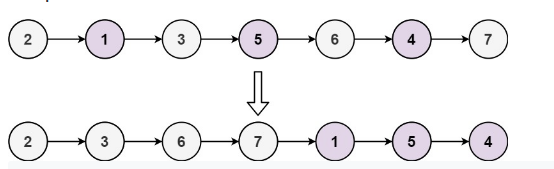
\includegraphics[scale=0.5]{images/oddEvenList.png}

\textbf{Entrada:} head = [2,1,3,5,6,4,7]

\textbf{Saída:} [2,3,6,7,1,5,4]


\begin{minted}{C++}

class ListNode {
    public:
    int val;
    ListNode *next;
    ListNode() : val(0), next(nullptr) {}
    ListNode(int x) : val(x), next(nullptr) {}
    ListNode(int x, ListNode *next) : val(x), next(next) {}

    
};


ListNode* oddEvenList(ListNode* head)
{
}
int main(){
    vector <int> v1({1,2,3,4,5});
    vector <int> v2({1,3,5,2,4});
    ListNode * head = toList(v1, 0, v1.size() - 1);
    head = oddEvenList(head);
    v1 = toVector(head);
    assert( v1 == v2 );
    return 0;    
}

\end{minted}


\item Dado o cabeça de uma lista encadeada simples ordenadas, exclua todas as duplicatas de forma que cada elemento apareça apenas uma vez. Retorne a lista encadeada ordenada também.

 
\textbf{Exemplo 1:}

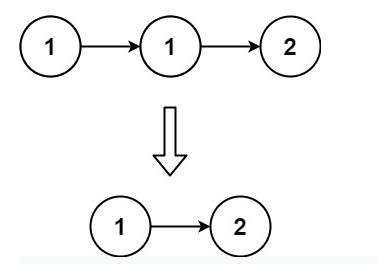
\includegraphics[scale=0.5]{images/deleteDuplicadas.png}


\textbf{Entrada:} head = [1,1,2]\\
\textbf{Saída:} [1,2]\\

\begin{minted}{C++}
class ListNode {
    public:
    int val;
    ListNode *next;
    ListNode() : val(0), next(nullptr) {}
    ListNode(int x) : val(x), next(nullptr) {}
    ListNode(int x, ListNode *next) : val(x), next(next) {}
};
ListNode* deleteDuplicates(ListNode* head) 
{
}
\end{minted}

\item Dados as cabeças de duas listas encadeadas, headA e headB, retorne o nó no qual as duas listas se cruzam. Se as duas listas encadeadas não tiverem nenhuma interseção, retorne nulo.

Por exemplo, as duas listas encadeadas a seguir começam a se cruzar no nó c1: 


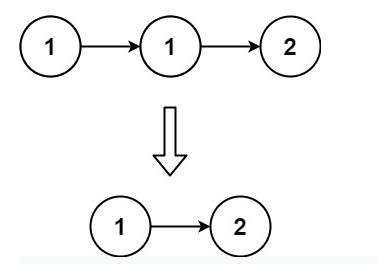
\includegraphics[scale=0.5]{images/deleteDuplicadas.png}

\textbf{Input:} headA = [4,1,8,4,5], headB = [5,6,1,8,4,5],

\textbf{Output:} list = [8,4,5]



\begin{minted}{C++}
class ListNode {
    public:
    int val;
    ListNode *next;
    ListNode() : val(0), next(nullptr) {}
    ListNode(int x) : val(x), next(nullptr) {}
    ListNode(int x, ListNode *next) : val(x), next(next) {}
};
ListNode *getIntersectionNode(ListNode *headA, ListNode *headB);
\end{minted}

\item Dada a cabeça de uma lista encadeada e um inteiro val, remova todos os nós da lista encadeada que possui Node.val == val e retorne a nova cabeça.

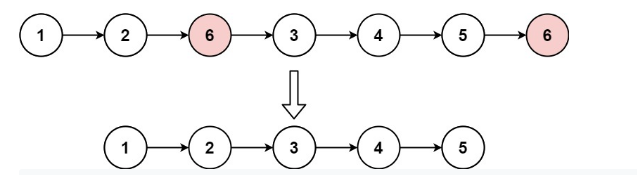
\includegraphics[scale=0.5]{images/removeElements.png}

Input: head = [1,2,6,3,4,5,6], val = 6

Output: [1,2,3,4,5]

\item Dado duas cabeças de duas listas encadeadas ordenadas, list1 e list2.

Mescle as duas listas em uma única lista ordenada. A lista deve ser feita juntando os primeiros nós das duas primeiras listas.

Retorne a cabeça da lista encadeada mesclada.

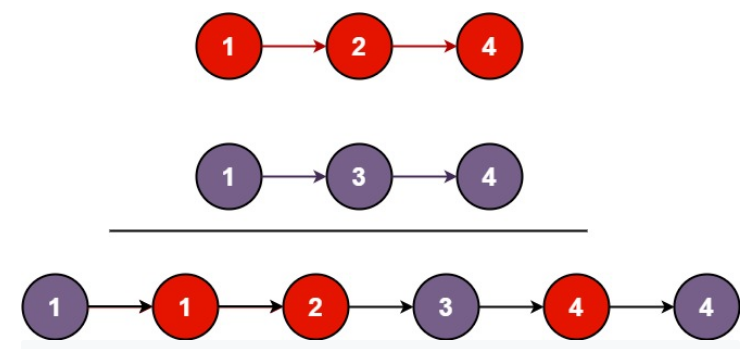
\includegraphics[scale=0.5]{images/mergelist.png}

Input: list1 = [1,2,4], list2 = [1,3,4]\\
Output: [1,1,2,3,4,4]\\

\item Dada a cabeça de uma lista encadeada simples, inverta a lista e retorne a lista invertida.

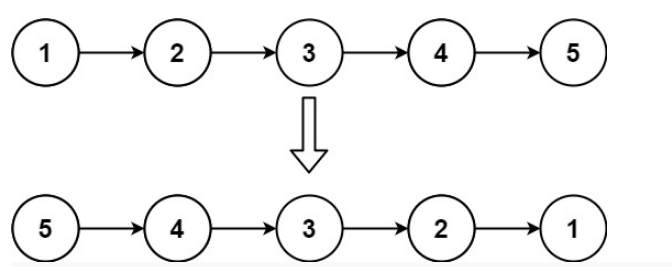
\includegraphics[scale=0.5]{images/reverseList.png}

Input: head = [1,2,3,4,5]\\
Output: [5,4,3,2,1]\\



\end{enumerate}


\section{Lista encadeada com descritores}

Um descritor de uma estrutura de dados é uma informação que ajuda a descrever a nossa estrutura e permite que algumas operações possam ser realizada de maneira mais eficiente.

A implementação da lista duplamente encadeada apresentada aqui possui os seguintes descritores:
\begin{itemize}
    \item Um nó sentinela chamado head que aponta para o primeiro elemento da nossa lista encadeada.
    \item Um nó sentinela chamado past\_last que é o próximo do último elemento da lista encadeada.
    \item a variável inteira count representando o tamanho da lista encadeada.
\end{itemize}

Observe que com esses descritores podemos facilmente adicionar um elemento no ínicio da lista encadeada e saber o tamanho da lista encadeada.

Além disso, temos duas classes aninhadas:

\begin{itemize}
    \item A classe Node que descreve o nó de uma lista encadeada.
    \item A classe Iterator utilizada para navegar pela lista encadeada sem expor sua representação interna.
\end{itemize}


\begin{listing}[!ht]
\caption{Definição da Lista encadeada simples com descritores}
\begin{minted}{C++}
template <typename T> 
class List{
    private:
        class Node;
        Node * head;
        Node * past_last;
        int count;
    public:        
        class Iterator;
        List() : count(0) { 
            head = new Node();
            past_last = new Node();
            head->next = past_last;
        }
        ~List(){   
        }    
        int size() { return count; }
        Iterator begin();
        Iterator before_begin();
        Iterator end();
        void pop_front();
        void insert_front(T val);
        T & front();
        void insert_after(Iterator it, T val); 
        void erase_after(Iterator it);
};
\end{minted}
\end{listing}

\begin{listing}[!ht]
\caption{Definição do nó de uma lista encadeada simples}
\begin{minted}{C++}
template <typename T>
class List<T>::Node{
    public:
    T val;
    Node * next;
    Node() : next(nullptr){}
    Node(T val, Node * ptr = nullptr) : val(val), next(ptr) {}
    
};
\end{minted}
\end{listing}

\begin{listing}[!ht]
\caption{Definição do iterador da lista encadeada simples}
\begin{minted}{C++}
template <typename T>
class List<T>::Iterator
{
    private:
    Node *atual;
    public:
    Iterator() : atual(nullptr){}
    
    Iterator(Node * atual) : atual(atual){ }
    
    Iterator next(){ return Iterator( atual->next); }
    
    T & value() { return atual->val; }
    
    bool operator!=(const Iterator & other) const{
        return atual != other.atual;
    }
    
    void insert_after(T val)
    {
        Node * ptr = new Node(val, atual->next);
        atual->next = ptr;
    }

    void erase_after()
    {
        Node * ptr = atual->next;
        atual->next = atual->next->next;
        delete ptr;
    }

};

\end{minted}
\end{listing}


\begin{listing}[!ht]
\caption{Definição dos métodos da lista encadeada simples}
\begin{minted}{C++}
template <typename T> 
T & List<T>::front()
{
    return head->next->val;
}
template <typename T> 
typename List<T>::Iterator List<T>::begin()
{
    return Iterator(head->next);
}
template <typename T> 
typename List<T>::Iterator List<T>::before_begin()
{
    return Iterator(head);
}
template <typename T> 
typename List<T>::Iterator List<T>::end()
{
    return Iterator(past_last);
}
template <typename T> 
void List<T>::pop_front(){
    if(count > 0){
        Node * ptr = head->next;
        head->next = head->next->next;
        count--;
        delete ptr;
    }
}
template <typename T> 
void List<T>::insert_front(T val)
{
    Node * ptr = new Node(val, head->next);
    head->next = ptr;
    count++;   
}
template <typename T> 
void List<T>::insert_after(Iterator it, T val)
{
    it.insert_after(val);
}
template <typename T> 
void List<T>::erase_after(Iterator it)
{
    it.erase_after();
}
\end{minted}
\end{listing}

% \section{STL List}

% Na STL do C++, temos dois tipos de listas:

% \begin{itemize}
%     \item forward\_list implementada como uma lista encadeada simples.
%     \item list implementada como uma lista duplamente encadeada.
% \end{itemize}

% \subsection{insertion\_sort}

% No código seguinte, comparamos insertion\_sort com a utilização de vector e list da STL.

% \begin{minted}{C++}
% #include <bits/stdc++.h>
% #include "debug.h"

% using namespace std;

% void insert(list <int> & l, int x){
%     auto it = l.begin();
%     for(; it != l.end(); ++it){
%         if(*it > x){
%             break;
%         } 
%     }
%     l.insert(it, x);
% }

% void insertion_sort(list <int> & l){
%     if(l.size() > 1){
%         int x = l.front();
%         l.pop_front();
%         insertion_sort(l);
%         insert(l, x);
%     }
% }

% void insert(vector<int> & v, int p, int r){
%     int x = v[p];
%     int j = p+1;
%     while( j <= r && v[j] < x){
%         v[j-1] = v[j];
%         j++;
%     }
%     v[j-1] = x;
% }


% void insertion_sort(vector <int> & v, int p,int r){    
%     if( r > p ){
%         int x = v[r];
%         insertion_sort(v, p+1, r);
%         insert(v, p, r);
%     }
% }


% vector <int> generate(int size, int limite_inferior = 0, int limite_superior = (int)1e9){
%     vector <int> output;
%     default_random_engine generator;
%     uniform_int_distribution<int> distribution(limite_inferior, limite_superior);

%     output.resize(size);
%     for(int i = 0; i < size; i++){
%         output[i] = distribution(generator);
%     }
%     return output;
% }



% int main(){

%     clock_t start, end;
%     vector <int> data = generate(10000, 0, 1000000);
    

%     list <int> l(data.begin(), data.end());
%     start = clock();
%     insertion_sort(l);
%     end = clock();
%     printf ("execution time %lf seconds.\n",((double) end-start)/CLOCKS_PER_SEC);
        
    
%     vector <int> A(data.begin(), data.end());
%     start = clock();
%     insertion_sort(A, 0 , A.size() - 1);
%     end = clock();
%     printf ("execution time %lf seconds.\n",((double) end-start)/CLOCKS_PER_SEC);    
% }

% //execution time 0.272482 seconds.
% //execution time 0.106265 seconds.


% \end{minted}

% Note que mesmo que com o tempo constante para a inserção e remoção da list da STL. O tempo de execução não é reduzido.


% \subsection{Josephus Problem}

% Nesta seção, vamos comparar três soluções para o problema Josephus:

% \begin{itemize}
%     \item JosephusArray: utiliza um array auxiliar para guardar as pessoas vivas, a operação de matar é realizada em tempo constante e a operação de buscar o próximo vivo é realizada em tempo linear.
%     \item JosephusVector: utiliza stl vector, a operação de matar é realizada em tempo linear e a operação de buscar o próximo vivo é realizada em tempo linear.
%     \item JosephusList: utiliza stl list, a operação de matar é realizada em tempo constante e a operação de buscar o próximo vivo é realizada em tempo constante.
% \end{itemize}


% \begin{center}
% \begin{tabular}{ccc}
% Implementação & matar & buscar o próximo vivo\\
% \hline 
% JosephusArray & $\mathcal{O}(1)$ & $\mathcal{O}(n)$\\
% JosephusVector & $\mathcal{O}(n)$ & $\mathcal{O}(1)$\\
% JosephusList & $\mathcal{O}(1)$ & $\mathcal{O}(1)$\\
% \end{tabular}
% \end{center}



% \begin{minted}{C++}

% #include <iostream>
% #include <bits/stdc++.h>
% using namespace std;

% int JosephusArray(int n, int k)
% {
%     k--;
%     int arr[n];
%     for (int i = 0; i < n; i++) {
%         arr[i] = 1; 
%     }
%     int cnt = 0, cut = 0, num = 1; // Cut = 0 gives the sword to 1st person.
%     while (cnt < (n - 1)) // Loop continues till n-1 person dies.
%     {
%         while (num <= k) // Checks next (kth) alive persons.
%         {
%             cut++;
%             cut = cut % n; // Checks and resolves overflow
%                           // of Index.
%             if (arr[cut] == 1) {
%                 num++; // Updates the number of persons
%                       // alive.
%             }
%         }
%         num = 1; // refreshes value to 1 for next use.
%         arr[cut] = 0; // Kills the person at position of 'cut'
%         if(num%100000==0)
%             printf("person %d died %d\n", num, cut );
%         cnt++; // Updates the no. of killed persons.
%         cut++;
%         cut = cut % n; // Checks and resolves overflow of Index.
%         while (arr[cut] == 0) // Checks the next alive person the
%                      // sword is to be given.
%         {
%             cut++;
%             cut = cut % n; // Checks and resolves overflow
%                           // of Index.
%         }
%     }
%     return cut + 1; // Output is the position of the last
%                     // man alive(Index + 1);
% }

% int JosephusVector(int n, int k){
%     vector <int> v;
%     for(int i = 0; i < n; i++)
%     {
%         v.push_back(i+1);
%     }

%     auto it = v.begin();

%     while(v.size()>1)
%     {
%         for(int i=1;i<k;i++)
%         {
%             it++;  
%             if(it==v.end()) it = v.begin();
%         }

%         it = v.erase(it);
          
%         if(it==v.end())
%         {
%             it = v.begin();
%         }
%     }
     
%     return v[0]; //returns front element of the list//
    



% }


% int JosephusList(int n, int k){
%     list<int>l; //creates a doubly linked list using stl container//
%     for(int i=0;i<n;i++)
%         l.push_back(i+1); //pushes i to the end of the doubly linked list//
      
%     auto it = l.begin(); 
%     while(l.size()>1){
         
%         for(int i=1;i<k;i++){
%             it++;
             
%             if(it==l.end()){
%               //if iterator reaches the end,then we change it to begin of the list//
%                 it = l.begin();
%             }
%         }

%         int num = n -l.size() + 1;    
%         if(num %100000 == 0)  
%         printf("person %d died %d\n", num , *it);

%          it = l.erase(it);
          
%          if(it==l.end()){
%           //if iterator reaches the end,then we change it to begin of the list//
%                 it = l.begin();
%             }
%     }
     
%     return l.front(); //returns front element of the list//
     
% }

% int main(){

%     int n = 1e5, k = 1e4, x;
%     clock_t start, end;

%     start = clock();
%     x = JosephusArray(n, k);
%     end = clock();
%     printf("sobrevivente %d\n", x);
%     printf("execution time %lf seconds.\n",((double) end-start)/CLOCKS_PER_SEC);

%     start = clock();
%     x = JosephusList(n, k);
%     end = clock();
%     printf("sobrevivente %d\n", x);
%     printf("execution time %lf seconds.\n",((double) end-start)/CLOCKS_PER_SEC);

%     start = clock();
%     x = JosephusVector(n, k);
%     end = clock();
%     printf("sobrevivente %d\n", x);
%     printf("execution time %lf seconds.\n",((double) end-start)/CLOCKS_PER_SEC);


%     return 0;

% }

% /*
% sobrevivente 45338
% execution time 41.915037 seconds.
% sobrevivente 45338
% execution time 7.246956 seconds.
% sobrevivente 45338
% execution time 9.671076 seconds.
% */
% \end{minted}




